\section{Phụ lục}

\subsection{Mô tả pipeline để tạo ra file Report.pdf}
Kết quả thực nghiệm của báo cáo này được thực hiện hoàn toàn thông qua Github Action, bằng hai repository sau:
\begin{itemize}
    \item \href{https://github.com/magnusdtd/sort-project/}{sort-project}
    \item \href{https://github.com/magnusdtd/sort-project-report/}{sort-project-report}
\end{itemize}

\begin{figure}[H]
    \centering
    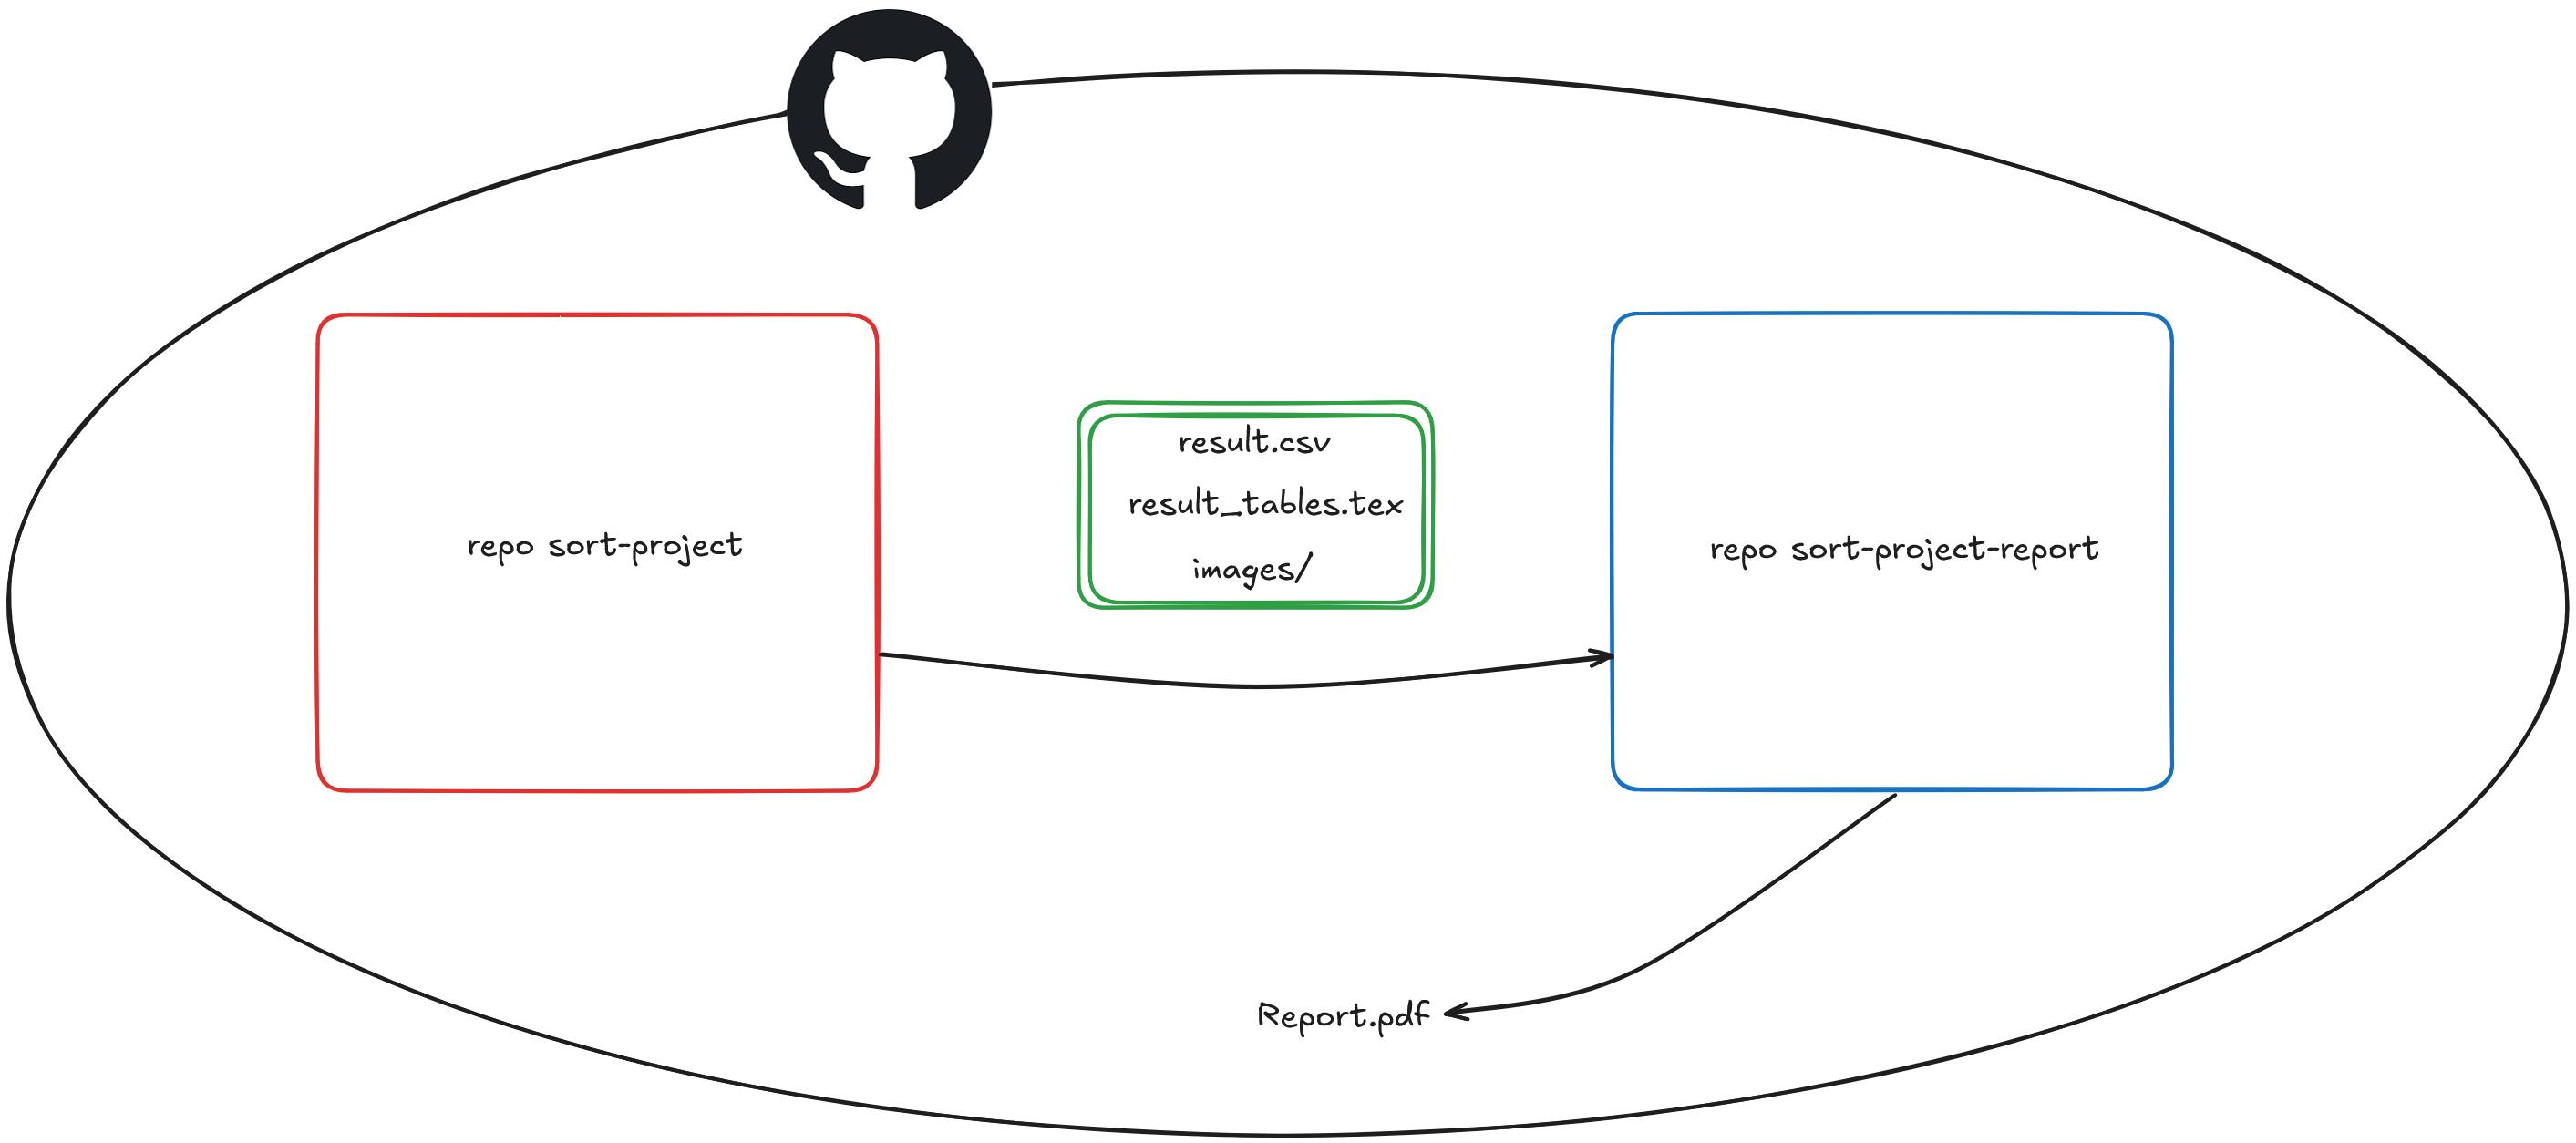
\includegraphics[width=\textwidth]{img/pipeline.png}
    \caption{Pipeline tạo ra số liệu cho thực nghiệm}
    \label{fig:pipeline}
\end{figure}

Pipeline này bao gồm hai file YAML chính:

\begin{itemize}
    \item \textbf{File YAML của repository sort-project}: File này được sử dụng để biên dịch, chạy và tạo release mới để chứa các file kết quả từ dự án C++ và Jupyter Notebook. Các bước chính bao gồm:
    \begin{itemize}
        \item Thiết lập môi trường MSVC và biên dịch file \texttt{run.cpp} thành \texttt{run.exe}.
        \item Chạy file \texttt{run.exe} để lấy được file \texttt{result.csv}.
        \item Thiết lập môi trường Python và cài đặt các thư viện cần thiết.
        \item Chạy Jupyter Notebook để chuyển file \texttt{result.csv} thành bảng latex và tạo ra các hình ảnh, biểu đồ cho báo cáo.
        \item Lưu trữ các file kết quả như \texttt{result.csv}, \texttt{result\_tables.tex} và thư mục \texttt{images}.
        \item Tạo một release mới trên GitHub và tải lên các file kết quả.
    \end{itemize}
    
    \item \textbf{File YAML của repository sort-project-report}: File này được sử dụng để biên dịch và tạo release mới để chứa file báo cáo. Các bước chính bao gồm:
    \begin{itemize}
        \item Tải các file \texttt{result.csv}, \texttt{result\_tables.tex} và thư mục \texttt{images} về từ release mới nhất của repository sort-project.
        \item Tải xuống và giải nén các file kết quả.
        \item Biên dịch tài liệu LaTeX thành file PDF.
        \item Đổi tên file PDF thành \texttt{Report.pdf}.
        \item Tạo một release mới trên GitHub và tải lên file \texttt{Report.pdf}.
    \end{itemize}
\end{itemize}

Với pipeline trên, việc chạy thực nghiệm nhiều lần trở nên dễ dàng mà không sợ nóng máy, cập nhật kết quả từ thực nghiệm thành báo cáo nhanh gọn, tiết kiệm thời gian hơn.